\section{Theorie}
\label{sec:Theorie}
Nach dem zweiten Hauptsatz der Thermodynamik kann Wärme nicht ohne äußere Arbeit aus einem Gebiet niedrigerer Temperatur in ein Gebiet höherer Temperatur übergehen. Will man diesen Vorgang umkehren, so lässt sich
eine \textbf{Wärmepumpe} verwenden. Mit ihr ist es möglich, Energie aus einem kälteren System in ein wärmeres zu übertragen. Dabei errechnet sich die an das wärmere Reservoir abgegebene Wärmemenge $Q_1$ 
aus der Summe der aufgewandten Arbeit $W$ und der dem kälteren Reservoir entzogenen Wärmemenge $Q_2$.

\begin{equation}
    \label{eq:q1ideal}
    Q_1= W + Q_2
\end{equation}

Dabei bezeichnet das Verhältnis von abgegebener Wärme und aufgewandter Arbeit die Güteziffer

\begin{equation}
    \label{eq:effideal}
    ν_{ideal} = \dfrac{Q_1}{W} \, \text{.}
\end{equation}

Unter der Annahme, dass es sich bei der Wärmeübertragung um einen vollständig reversiblen Prozess handelt und dass sich die Temperaturen der Reservoire während des Prozesses näherungsweise nicht ändern, lässt sich aus
$\int{\mathrm{dQ}\dfrac{1}{T_i}}=0$ die Beziehung

\begin{equation}
    \label{eq:rever}
    \dfrac{Q_1}{T_1} - \dfrac{Q_2}{T_2} = 0
\end{equation}
herleiten.
Daraus lässt sich nun mit \eqref{eq:q1ideal}

\begin{equation}
    Q_1 = W +\dfrac{T_2}{T_1}Q_1
\end{equation}
    
folgern und es ergibt sich aus \eqref{eq:effideal}
\begin{equation}
    ν_{ideal} = \dfrac{Q_1}{W} = \dfrac{T_1}{T_1-T_2} \, \text{.} \label{eq:effTdiff}
\end{equation}

\newpage

Dabei ist aber zu beachten, dass es sich bei den hier aufgeführten Gleichungen lediglich um idealisierte Annahmen handeln, die aufgrund unvermeidbarer Verluste realer Wärmepumpen nicht verhindert werden können.
Für reale Wärmepumpen gilt lediglich

\begin{align}
    \dfrac{Q_1}{T_1} - \dfrac{Q_2}{T_2} > 0 \\
    ν_{real} < \dfrac{T_1}{T_1-T_2} \text{.} \label{eq:effreal}
\end{align}

Wie sich an \eqref{eq:effTdiff} und \eqref{eq:effreal} erkennen lässt, arbeiten Wärmepumpen deutlich effizienter, wenn die Temperaturdifferenz der einzelnen Reservoire möglichst gering ist, da so der Nenner $T_1-T_2$
gegen $0$ konvergiert und der Ausdruck somit gegen $\infty \,$ geht. Daraus folgt aber gleichzeitig, dass die Pumpe mit voranschreitender Zeit und somit wachsender Temperaturdifferenz ineffizienter wird. Je wärmer also
Reservoir 1 und je kälter Reservoir 2, desto mehr Arbeit muss aufgewandt werden, um Reservoir 1 weiter zu erhitzen.

\subsection{Funktionsweise und Aufbau einer Wärmepumpe}

\begin{figure}
    \centering
    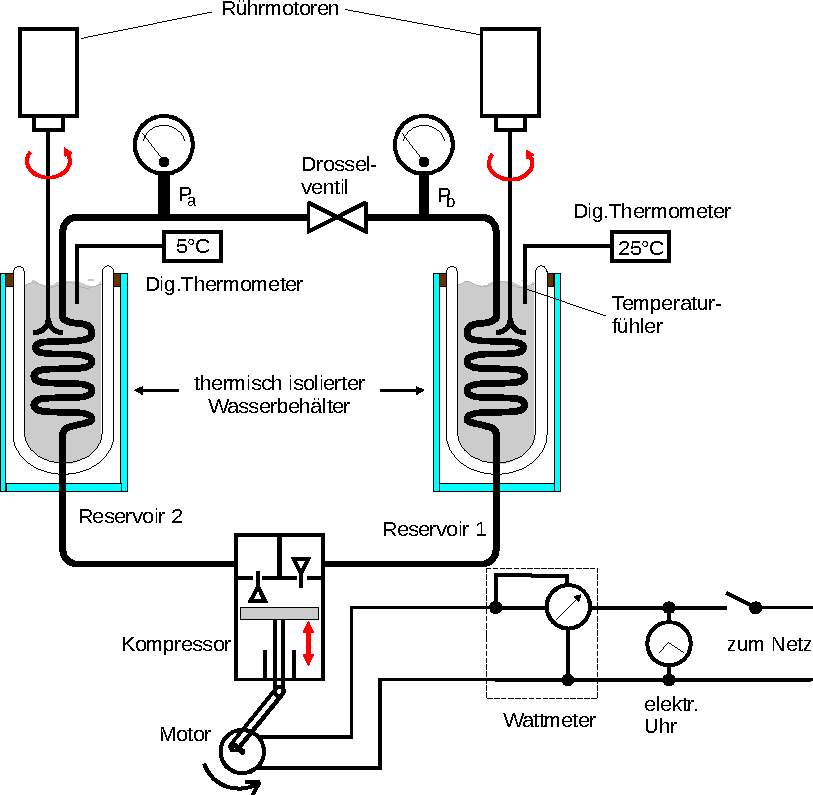
\includegraphics[scale=0.7]{Abb_1.pdf}
    \caption{Schematische Darstellung einer Wärmepumpe \cite{ap02}.} 
    \label{fig:abb1}
\end{figure}

Die Wärmepumpe nutzt die Eigenschaft von Stoffen, der Umgebung beim Verdampfen Wärme zu entziehen und diese beim Kondensieren wieder an seine Umgebung abzugeben, um den Wärmetransport vom kälteren in das wärmere Reservoir
zu ermöglichen. Das dazu verwendete Gas sollte dabei eine möglichst hohe Kondensationswärme besitzen. Der Kreislauf wird dabei vom Kompressor in Gang gesetzt, das Gas durchströmt das Drosselventil und die Reservoire.
Aufgrund des hohen Strömungswiderstandes am Drosselventil baut sich eine Druckdifferenz $p_b-p_a$ auf.
Die Pumpe ist dabei so aufgebaut, dass das Gas in Reservoir 1 der Temperatur $T_1$ und dem Druck $p_b$ flüssig und in Reservoir 2 der Temperatur $T_2$ und dem Druck $p_a$ mit $T_1 > T_2$ und $p_b > p_a$ gasförmig ist.
Das bei $p_b$ verflüssige Gas verdampft nach dem Eintritt in Reservoir 2 und entzieht diesem Wärme, woraufhin es im Kompressor komprimiert wird und anschließend in Reservoir 1 wieder flüssig wird und die aufgenomme Wärme
an dieses abgibt.

\subsection{Bestimmung wichtiger Kenngrößen}

Zur genauen Auswertung des Versuches ist die Bestimmung einiger Kenngrößen der Wärmepumpe notwendig.

\subsubsection{Bestimmung von $ν_{real}$}

Für die reale Güteziffer $ν_{real}$ gilt

\begin{equation}
    ν_{real} = \dfrac{ΔQ_1}{ΔtN},
\end{equation}
wobei $N$ die über das Zeitintervall $Δt$ gemittelte Leistungsaufnahme des Kompressors, die am Wattmeter angezeigt wird, darstellt. 
Der Differenzenquotient $\dfrac{ΔQ_1}{Δt}$ beschreibt dabei die im Zeitintervall gewonnene Wärmemenge $Q_1$. Er ergibt sich zu

\begin{equation}
    ν_{real} = \dfrac{ΔQ_1}{ΔtN} = (m_1c_w + m_kc_k)\dfrac{ΔT_1}{ΔtN}
    \label{eq:effrealdiffquo}
\end{equation}

\subsubsection{Bestimmung des Massendurchsatzes}

Analog zu \eqref{eq:effrealdiffquo} lässt sich auch der Differenzenquotient $\dfrac{ΔQ_2}{Δt}$, als Reservoir 2 im Intervall $Δt$ entnommene Wärmemenge $Q_2$, und damit der Massendurchsatz berechnen.
Es gilt

\begin{equation}
    \label{eq:Massendurch}
    \dfrac{ΔQ_2}{Δt} = (m_2c_w +m_kc_k)\dfrac{ΔT_2}{Δt}.
\end{equation}

Ist nun die Verdampfungswärme $L\dfrac{Δm}{Δt}$, ergibt sich

\begin{equation}
    \dfrac{Δm}{Δt} = \dfrac{1}{L}\dfrac{ΔQ_2}{Δt}.
    \label{eq:Massendurch2}
\end{equation}

\newpage

\subsubsection{Bestimmung der machanischen Kompressorleistung $N_{mech}$}

Für die Verringerung eines Gasvolumens von $V_a$ auf $V_b$ gilt für die Arbeit des Kompressors allgemein

\begin{equation}
    A_m= -\int_{V_a}^{V_b} p \, \text{d}V.
\end{equation}

Unter der Annahme, dass die Kompression des Gases näherungsweise adiabatisch verlaufe, gilt für den Zusammenhang zwischen Druck und Volumen nach der Poissonschen Gleichung

\begin{equation}
    p_aV_a^κ=p_bV_b^κ=pV^κ
\end{equation}
mit dem Verhältnis $κ > 1$ der molaren und spezifischen Wärmekapazitäten $c_p$ und $c_v$.

Daraus lässt sich folgern

\begin{equation}
    A_m=-p_aV_a^κ\int_{V_a}^{V_b} V^{-κ} \text{d}V = 
    \dfrac{1}{κ-1}p_aV_a^κ \left (V_b^{κ-1}-V_a^{-κ+1} \right)= \dfrac{1}{κ-1} \left(p_b\left(\dfrac{p_a}{p_b}\right)^{\dfrac{1}{κ}}-p_a\right)V_a
     \nonumber
\end{equation}
und für die Kompressorleistung

\begin{equation}
    \label{eq:kompressorleistung}
    N_{mech}= \dfrac{ΔA_m}{Δt} = \dfrac{1}{κ-1} \left(p_b\left(\dfrac{p_a}{p_b}\right)^{\dfrac{1}{κ}}-p_a\right) \dfrac{ΔV_a}{Δt} = 
    \dfrac{1}{κ-1} \left (p_b \left(\dfrac{p_a}{p_b} \right)^{\dfrac{1}{κ}}-p_a \right) \dfrac{1}{ρ}\dfrac{Δm}{Δt},
\end{equation}
wobei $ρ$ die Gasdichte beim Druck $p_a$ darstellt.
    

